\documentclass[onecolumn,aps, pre,amsmath,amssymb,longbibliography,11pt]{revtex4-2}
\usepackage{graphicx}
% \usepackage{dcolumn}
\usepackage{bm}
\usepackage{amsfonts}
\usepackage{xcolor,tabu}
\usepackage{multirow}
\usepackage{amsthm}
\usepackage{textcomp}
\usepackage{tikz}
\usepackage[colorlinks=true,
            linkcolor=blue,
            urlcolor=blue,
            citecolor=blue]{hyperref}
\hypersetup{bookmarksopen=true}
\usepackage{xr}
\usepackage{float}



\begin{document}
\title{Description of the cross-correlaiton functions in Fig. 5C}

% \author{Zhengyang Liu}
% \date{\today}
\maketitle

The 3 cross-correlation functions in Fig.~5C in the main text are described below.

\begin{figure}[h]
  \begin{center}
    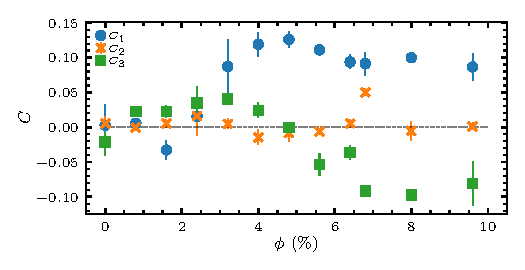
\includegraphics[width=5in]{cross-correlations.pdf}
  \end{center}
  \caption[]{Figure 5C in main text.}
  \label{fig:orientation}
\end{figure}



$C_1$ is the cross-correlation function between local density fluctuation $\delta N$ and kinetic energy $E$.
$C_1$ shown in Fig.~5C is an average over 1000 single frame correlation $C_1'$, and $C_1'$ is defined as
\begin{equation}
  C_1' = \frac{ \langle (\delta N-\overline{\delta N})(E-\overline E) \rangle }{\sigma_{\delta N}\sigma_E}
\end{equation}
$C_2$ is the cross-correlation function between local density $N$ and divergence of bacterial flux $\nabla\cdot(N\bm{v})$.
$C_3$ is the cross-correlation function between local density $N$ and kinetic energy $E$.
$C_2'$ and $C_3'$ are single frame correlations similar to $C_1'$, and are defined as
\begin{equation}
  C_2' = \frac{ \langle (N-\overline{N})(\nabla\cdot(N\bm{v})-\overline{\nabla\cdot(N\bm{v})} ) \rangle }{\sigma_{N}\sigma_{\nabla\cdot(N\bm{v})}}
\end{equation}
\begin{equation}
  C_3' = \frac{ \langle (N-\overline N)(E-\overline E) \rangle }{\sigma_N\sigma_E}
\end{equation}
$\overline A$ indicates the mean of variable $A$, $\sigma_A$ indicates the standard deviation of A, and $\langle A \rangle$ denotes the average of A over all the positions.
\end{document}
